\documentclass[12pt, a4paper]{article}
\usepackage[utf8]{inputenc}
\usepackage[english]{babel}
\usepackage{amsmath}
\usepackage{amsfonts}
\usepackage{amssymb}
\usepackage{csquotes}
\usepackage{mathtools}
\usepackage{graphicx}
\usepackage{geometry}
\usepackage{setspace}
\usepackage{longtable}
\usepackage{float}
\usepackage{comment}
\usepackage{listings}
\usepackage{minted}
\usepackage{fancyhdr}
\usepackage{blindtext}
\usepackage{siunitx}
\usepackage[colorlinks=true, allcolors=blue]{hyperref}

\usepackage[style=authoryear]{biblatex}
\addbibresource{Bibliography.bib}

\geometry{top = 2.5cm, bottom = 2.5cm, left= 3cm, right= 3cm}

\fancypagestyle{mystyle}
{
    \rhead{Experiment 6}
    \lfoot{Lee Farrugia}
    \cfoot{}
    \rfoot{Page \thepage}
    \renewcommand{\headrulewidth}{0pt}
    \renewcommand{\footrulewidth}{0.5pt}
}

\fancypagestyle{titlepagestyle}
{
    \fancyhf{}
    \lfoot{Lee Farrugia}
    \cfoot{}
    \rfoot{Page \thepage}
    \renewcommand{\headrulewidth}{0pt}
    \renewcommand{\footrulewidth}{0.5pt}
}

\title{The linear expansion of solids}
\author{Lee Farrugia \\ Experiment 6 \\ Group 1A}

\date{8$^{\text{th}}$ April 2022}

\begin{document}

\maketitle
\thispagestyle{titlepagestyle}
\pagestyle{mystyle}

\section*{Aim}
The aim of this experiment was to determine the coefficient of linear expansion of the material and from this determine what material being used is. 

\section*{Diagram}
\begin{figure}[H]
    \centering
    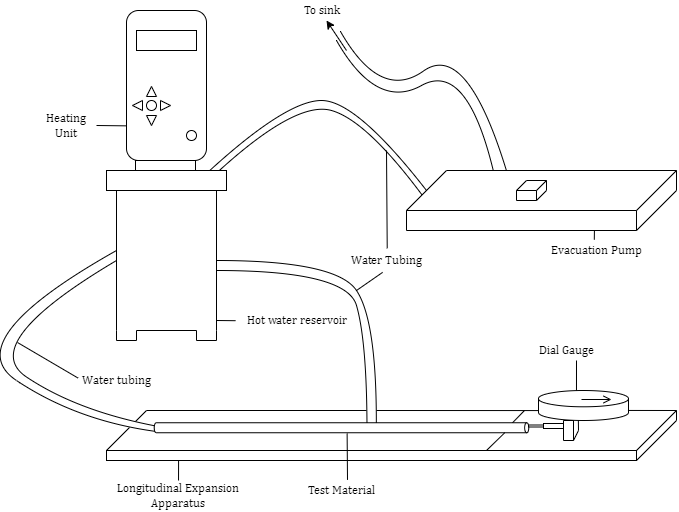
\includegraphics[width = \textwidth]{Experiment 6.png}
    \caption{Set Up}
    \label{fig: Apparatus}
\end{figure}

\section*{List of Apparatus}
Heating unit, pump, piping, test material, dial gauge, longitudinal expansion apparatus, beaker, sink.

\section*{Language and Packages}
Python 3.9.7, Matplotlib.pyplot, Numpy, Pandas, Sympy, Math

\section*{Procedure}
\begin{enumerate}
    \item The original length of the tube was measured and noted in the table below.
    \item The dial gauge was adjusted so to ensure the initial position is set as zero.
    \item The reservoir was filled between half and three quarters full. It was made sure that the heating element and the pump inlet were completely immersed by the water.
    \item The heating unit was switched on, both from the mains and from the back switch.
    \item The temperature, $\theta$, on the heating element was set to \qty{35}{\degreeCelsius} and noted below. The heater was started.
    \item The temperature was allowed to settle before reading the change in length, $\Delta l$. The range of change of the temperature was also noted.
    \item The expansion length was noted in the table below.
    \item The temperature was increased in steps of \qty{5}{\degreeCelsius} up to \qty{85}{\degreeCelsius}.
    \item The procedure was repeated for the cooling cycle where the temperature was decreased by step of \qty{5}{\degreeCelsius}. The heating unit was assisted by pumping some of the hot water out from the reservoir and refilled with water from the beaker.
    \item This procedure was repeated for another heating and cooling cycle.
\end{enumerate}

\section*{Precautions}
\begin{itemize}
    \item[-] The temperature was allowed to somewhat stabilise before taking the reading of the expansion length.
    \item[-] Repeated readings of the expansion length at each temperature point were taking.
    \item[-] The variation range of the temperature was noted each time at each temperature point.
    \item[-] When pumping out hot water from the reservoir it was done in short bursts and the water was replaced slowly.
    \item[-] It was made sure that the heating element and the pump inlet were always covered throughout the experiment.
\end{itemize}

\section*{Sources of Error}
\begin{itemize}
    \item[-] The material may have had impurities.
    \item[-] The rod of the material may have not been uniform.
    \item[-] Temperature changes in the material due to heat loss to atmosphere.
    \item[-] Draught created by walking student and instructors in the laboratory.
    \item[-] The dial gauge may have not been perfectly aligned with the centre of the rod.
\end{itemize}

\section*{Data and Graphs}
\begin{longtable}{|c|c|c|c|c|}
\hline
$l_0/\text{ m}$ & \textpm 0.001 & 0.399 & 0.400 & 0.399\\ \hline
\caption{Original length readings}
\label{Tab : Table 1}\\
\end{longtable}

\begin{longtable}{|c|c|c|c|c|c|c|c|c|c|c|c|}
\hline
$H_1$/$^{\circ}$C & $dl_1$/m & $C_1$/$^{\circ}$C & $dl_2$/m & $H_2$/$^{\circ}$C & $dl_3$/m & $C_2$/$^{\circ}$C & $dl_4$/m\\ \hline
\textpm 0.01 & \textpm 0.0001 & \textpm 0.01 & \textpm 0.0001 & \textpm 0.01 & \textpm 0.0001 & \textpm 0.01 & \textpm 0.0001 \\ \hline
\endfirsthead

\hline
$H_1$/$^{\circ}$C & $dl_1$/m & $C_1$/$^{\circ}$C & $d2_1$/m & $H_2$/$^{\circ}$C & $d3_1$/m & $C_2$/$^{\circ}$C & $d4_1$/m\\ \hline
\textpm 0.01 & \textpm 0.0001 & \textpm 0.01 & \textpm 0.0001 & \textpm 0.01 & \textpm 0.0001 & \textpm 0.01 & \textpm 0.0001 \\ \hline
\endhead

35.00 & 0.0007 & 35.00 & 0.0006 & 35.00 & 0.0006 & 35.00 & 0.0006\\ \hline
40.00 & 0.0008 & 40.00 & 0.0008 & 40.00 & 0.0008 & 40.00 & 0.0008\\ \hline
45.00 & 0.0011 & 45.00 & 0.0011 & 45.00 & 0.0011 & 45.00 & 0.0011\\ \hline
50.00 & 0.0014 & 50.00 & 0.0013 & 50.00 & 0.0013 & 50.00 & 0.0013\\ \hline
55.00 & 0.0016 & 55.00 & 0.0015 & 55.00 & 0.0015 & 55.00 & 0.0015\\ \hline
60.00 & 0.0018 & 60.00 & 0.0018 & 60.00 & 0.0018 & 60.00 & 0.0017\\ \hline
65.00 & 0.0021 & 65.00 & 0.0020 & 65.00 & 0.0020 & 65.00 & 0.0020\\ \hline
70.00 & 0.0023 & 70.00 & 0.0023 & 70.00 & 0.0023 & 70.00 & 0.0023\\ \hline
75.00 & 0.0025 & 75.00 & 0.0025 & 75.00 & 0.0025 & 75.00 & 0.0025\\ \hline
80.00 & 0.0027 & 80.00 & 0.0027 & 80.00 & 0.0027 & 80.00 & 0.0027\\ \hline
85.00 & 0.0030 & 85.00 & 0.0030 & 85.00 & 0.0029 & 85.00 & 0.0030\\ \hline
\caption{Temperature and Expansion length readings}
\label{Tab : Table 2}\\
\end{longtable}

\begin{longtable}{|c|c|c|c|c|c|c|c|}
\hline
$H_1$/$^{\circ}$C & $dt_1$/m & $C_1$/$^{\circ}$C & $dt_2$/m & $H_2$/$^{\circ}$C & $dt_3$/m & $C_2$/$^{\circ}$C & $dt_4$/m\\ \hline
\textpm 0.01 & \textpm 0.01 & \textpm 0.01 & \textpm 0.01 & \textpm 0.01 & \textpm 0.01 & \textpm 0.01 & \textpm 0.01 \\ \hline
\endfirsthead

\hline
$H_1$/$^{\circ}$C & $dt_1$/m & $C_1$/$^{\circ}$C & $dt_2$/m & $H_2$/$^{\circ}$C & $dt_3$/m & $C_2$/$^{\circ}$C & $dt_4$/m\\ \hline
\textpm 0.01 & \textpm 0.01 & \textpm 0.01 & \textpm 0.01 & \textpm 0.01 & \textpm 0.01 & \textpm 0.01 & \textpm 0.01 \\ \hline
\endhead

35.00 & 0.03 & 35.00 & 0.03 & 35.00 & 0.03 & 35.00 & 0.03\\ \hline
40.00 & 0.08 & 40.00 & 0.08 & 40.00 & 0.09 & 40.00 & 0.05\\ \hline
45.00 & 0.11 & 45.00 & 0.03 & 45.00 & 0.12 & 45.00 & 0.02\\ \hline
50.00 & 0.13 & 50.00 & 0.08 & 50.00 & 0.17 & 50.00 & 0.09\\ \hline
55.00 & 0.18 & 55.00 & 0.10 & 55.00 & 0.24 & 55.00 & 0.10\\ \hline
60.00 & 0.21 & 60.00 & 0.16 & 60.00 & 0.30 & 60.00 & 0.17\\ \hline
65.00 & 0.23 & 65.00 & 0.08 & 65.00 & 0.39 & 65.00 & 0.08\\ \hline
70.00 & 0.24 & 70.00 & 0.11 & 70.00 & 0.24 & 70.00 & 0.11\\ \hline
75.00 & 0.34 & 75.00 & 0.29 & 75.00 & 0.40 & 75.00 & 0.13\\ \hline
80.00 & 0.47 & 80.00 & 0.43 & 80.00 & 0.59 & 80.00 & 0.43\\ \hline
85.00 & 0.51 & 85.00 & 0.55 & 85.00 & 0.63 & 85.00 & 0.51\\ \hline
\caption{Temperature and Temperature variation}
\label{Tab : Table 3}
\end{longtable}

Graph is on page \pageref{fig: plot1}.

\begin{figure}
    \centering
    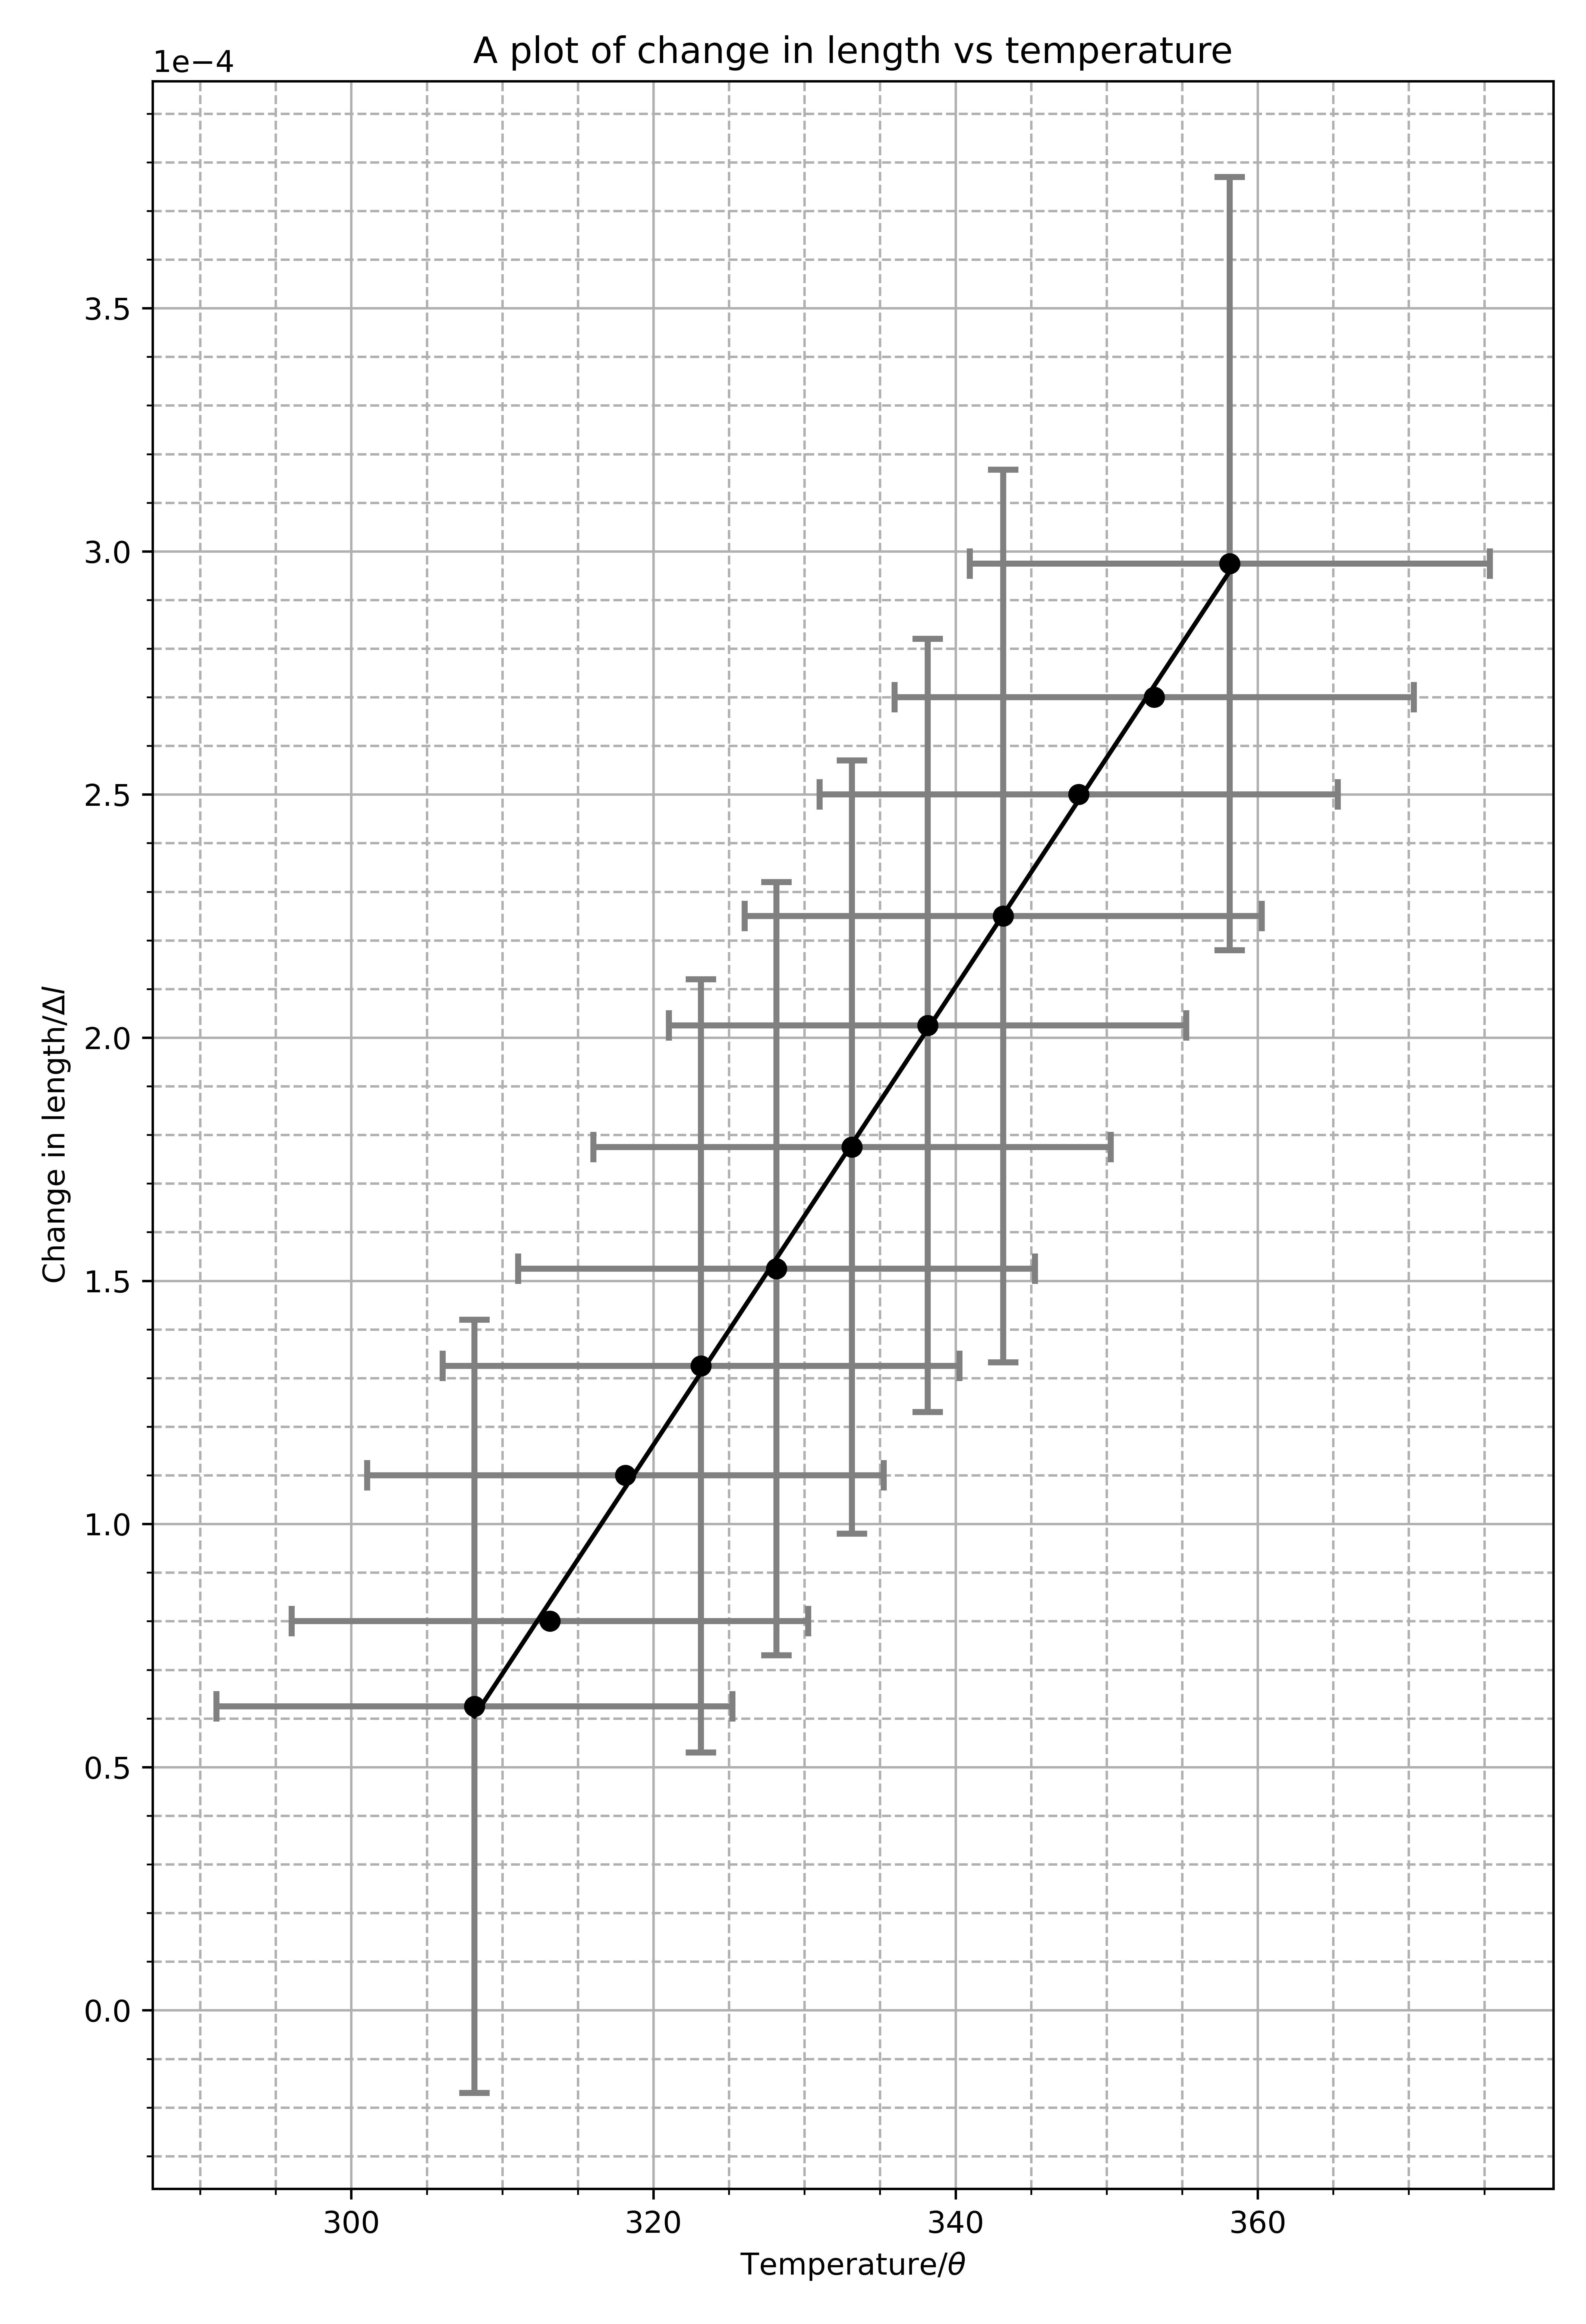
\includegraphics[width = \textwidth]{Plot1.png}
    \caption{Change in Length vs temperature}
    \label{fig: plot1}
\end{figure}

\section*{Calculations}
The data gathered during the experiment was read by the program using the following line of code:
\begin{lstlisting}
    data = pd.read_excel(`Experiment 6.xlsx') .
\end{lstlisting}
The temperature readings, expansion readings were inputted by the following lines of code:
\begin{lstlisting}
    temp = (np.asarray(data[`heating 1'] + data[`cooling 1'] +
       data[`heating 2'] + data[`cooling 2'])/4) + 273.15
    dl = np.asarray(data[`dl1'] + data[`dl2'] + 
     data[`dl3'] + data[`dl4'])/40 ,
\end{lstlisting}
where $temp$ corresponds to the temperatures of the heating cooling cycles, and $dl$ corresponds to the expansion at each temperature. The original length of the rod was measured and denoted as $l_0$ and inputted into the program by the following lines of code:
\begin{lstlisting}
    l0 = np.asarray(data[`l'])
    l0 = l0[~np.isnan(l0)]
    l0a = np.average(l0) .
\end{lstlisting}
The equation given was $l=l_0(1+\alpha\Delta\theta)$, which was rearranged as follows:
\begin{align*}
    l-l_0&=l_0(\alpha\theta-\theta_0)\\
    dl&=l_0\alpha\theta-l_0\theta_0\,,
\end{align*}
where $l$ is the final length, $l_0$ is the original length, $dl$ is the change in length, $\alpha$ is the coefficient of linear expansion, $\theta$ is the current temperature, $\theta_0$ is the original temperature. Therefore on comparing with the straight line equation $y=mx+c$ it can be noted that $dl$ corresponds with $y$ and $theta$ corresponds with $x$, thus making $l_0\alpha$ corresponding with the gradient $m$. Thus, $dl$ was plotted against $temp$ in order to obtain the straight line needed. This was done with the following lines of code:
\begin{lstlisting}
    Y = dl
    X = temp
    coeffs, cov = np.polyfit(X, Y, deg=1, cov=True)
    poly_func = np.poly1d(coeffs)
    trendline = poly_func(X) ,
\end{lstlisting}
First the program found the coefficients of the line of best for the data inputted which then were used to produce the line by substituting the $x$-axis values into the equation. From this by calling the correct position in the coeffs array and dividing by the value of $l_0$, the value of $\alpha$ was found to be 1.18$\times10^{-5}$ K$^{-1}$. In order to find the error of the value of $\alpha$ the following equation was used:
\begin{align*}
    \alpha &= \frac{m}{l_0}\,,\\
    \Delta\alpha &= \sqrt{{\frac{\partial \alpha}{\partial m}}^2\Delta l_0 + {\frac{\partial \alpha}{\partial l_0}}^2 \Delta m}\,,
\end{align*}
this was done through the following line of code:
\begin{lstlisting}
    def merror(c, d, dm, dl0):
        a = Symbol(`a')
        b = Symbol(`b')
        equation = a/b
        diff_a = Derivative(equation, a)
        diff_b = Derivative(equation, b)
        da = diff_a.doit()
        db = diff_b.doit()
        dc = da.subs({a : c, b : d}).evalf()
        dd = db.subs({a : c, b : d}).evalf()
        return (dc*dm)**2 + (dd*dl0)**2
    err = sqrt(merror(m, l0a, dm, dl0)) .
\end{lstlisting}
Therefore the value of $\alpha$ was found to be $1.18\times10^{-5}\pm1.01\times10^{-7}$ K$^{-1}$. In order to create the error bars as can be seen in the graph, the variation of each reading had to be calculated. For the expansion lengths, the standard deviation was calculated using the following equation:
\begin{equation*}
    \Delta x = t_{\alpha,n-1} \times \frac{s}{\sqrt{n}}\,,
\end{equation*}
this was done using the following lines of code:
\begin{lstlisting}
    dYstd = np.std([data[`dl1'], data[`dl2'], 
        data[`dl3'], data[`dl4']], axis=0, ddof=1) 
    dY = (3.18/np.sqrt(4)) * dYstd
    dX = 0.25 * (np.asarray(data[`dt1'] + data[`dt2'] + 
        data[`dt3'] + data[`dt4']) + 273.15)/4 .
\end{lstlisting}
In the case of the temperature variation it should be noted that code used for the error bars corresponds to the following equation:
\begin{equation*}
    \Delta T = 3.18 \times \frac{\frac{dt_1 + dt_2 + dt_3 + dt_4}{4}}{\sqrt{4}}\,.
\end{equation*}
The accuracy and precision of the obtained values were found using the following equations:
\begin{align*}
    \text{Accuracy} &= \frac{\text{Experimental Value}}{\text{Actual Value}} \times 100\% \\
    \\
    \text{Precision}&=\frac{\text{Combined Error}}{\text{Experimental Value}} \times 100\% \,,
\end{align*}
this was done with the following code:
\begin{lstlisting}
    precision = (err/(coeffs[0]/l0a))*100
    accuracy = (((coeffs[0]/l0a)/(11e-6)))*100,
\end{lstlisting}
the accuracy was found to be 7.20\% while the precision was 0.94\%.

\section*{Discussion}
The coefficient of linear expansion was found to be \num{1.18d-5} \textpm \qty{1.01d-5}{\kelvin^{-1}} which corresponds closely to the \qty{1.1d-5}{\kelvin^{-1}} given in the lab report, therefore it was concluded that the material used was steel. The accuracy of the results obtained was found to be $7.20\%$ and the precision of the data collected was found to be $0.94\%$. This indicates that the result obtained was quite accuracy when compared to the real value, while the data was gathered in a quite precise manner. This can be attributed in the precautions taken while doing the experiment. This is accuracy and precision is further highlighted by the fact that the error bars in the graph are quite small when taking into consideration the scale being used on the axis.

\medskip
\noindent
When a solid is above absolute zero its atoms are oscillating about their equilibrium position as they have a fixed amount of kinetic and potential energy. However, upon heating the atom will gain more energy thus, increasing their kinetic energy and potential energy, therefore they would take up more space as their oscillation around their equilibrium position increases in range \parencite{muncaster}.

\smallskip
\noindent
Thermal expansion is a fundamental property of solids, however, not all solids will expand when heated. Certain material such as metallic oxides, Invar alloys, cyanide polymers will contract on heating. This is referred as negative thermal expansion \parencite{miller2009negative}. Usually the the materials are split into three categories: (i) flexible network, (ii) atomic radius contraction and (iii) magnetovolume effect \parencite{NTE}. Materials that are part of the flexible network category , the atom latices will rearrange themselves to occupy less space upon heating thus making the material have a negative thermal expansion. The materials that make up the atomic radius contraction category will transfer a charge from one atom to another upon heating. The atom donating the electron would shrink in size while the atom receiving the electron will expand, in order for negative thermal expansion to happen the change in radius when donating the electron must be much larger than the change in radius when receiving the electron \parencite{NTE}. The materials making up the magnetovolume effect category show a magnetic preference when having a large volume. This was explained by Guillaume, as when the volume increases it would suppress the overlap of electronic orbitals and therefore reducing the width of electronic bands. This creates an increase in density which favours the creation of magnetic moments \parencite{NTE}.

\section*{References}
\printbibliography[heading=none]


\section*{Appendix}
\lstset{language=Python,
    showstringspaces=false,
    showtabs=false}
\begin{lstlisting}
import pandas as pd
import numpy as np
import matplotlib.pyplot as plt
from sympy import *
from math import sqrt

#importing the data
data = pd.read_excel(`Experiment 6.xlsx')
#defining constants
temp = (np.asarray(data[`heating 1'] + data[`cooling 1'] +
       data[`heating 2'] + data[`cooling 2'])/4) + 273.15
dl = np.asarray(data[`dl1'] + data[`dl2'] + 
     data[`dl3'] + data[`dl4'])/40
l0 = np.asarray(data[`l'])
l0 = l0[~np.isnan(l0)]
l0a = np.average(l0)

#defining the y and x axis
Y = dl
X = temp

#defining the variation of each constant
dl0 = 4.30 * np.std(data[`l'])/np.sqrt(3)
dYstd = np.std([data[`dl1'], data[`dl2'], 
        data[`dl3'], data[`dl4']], axis=0, ddof=1)
dY = (3.18/np.sqrt(4)) * dYstd
dX = 0.25 * (np.asarray(data[`dt1'] + data[`dt2'] + 
     data[`dt3'] + data[`dt4']) + 273.15)/4

#defining the straight line to be plotted
coeffs, cov = np.polyfit(X, Y, deg=1, cov=True)
poly_func = np.poly1d(coeffs)
trendline = poly_func(X)
m = coeffs[0]
dm = np.sqrt(cov[0][0])

#finding the error of the coefficient
def merror(c, d, dm, dl0):
    a = Symbol(`a')
    b = Symbol(`b')
    equation = a/b
    diff_a = Derivative(equation, a)
    diff_b = Derivative(equation, b)
    da = diff_a.doit()
    db = diff_b.doit()
    dc = da.subs({a : c, b : d}).evalf()
    dd = db.subs({a : c, b : d}).evalf()
    return (dc*dm)**2 + (dd*dl0)**2

err = sqrt(merror(m, l0a, dm, dl0))
print(f`The thermal coefficient of the material is 
        {coeffs[0]/l0a:.2e}K\u207b\u00b9 \u00b1 
        {err:.2e}K\u207b\u00b9 ')
        
#defining the precision and accuracy
precision = (err/(coeffs[0]/l0a))*100
accuracy = (((coeffs[0]/l0a)/(11e-6)))*100
print(f`The accuracy is {accuracy:.2f}% and 
        the precision is {precision:.2f}%')

#defining the plot size and axis
plt.figure(figsize=(7.3, 10.7))
plt.ticklabel_format(axis=`y', style=`sci', scilimits=(0,0))
plt.xticks(X)

#plotting the error bars
plt.errorbar(X, Y, xerr=dX, yerr=dY, fmt=`o', 
             color=`k', elinewidth=2, capthick=2, capsize=5,
             ecolor=`grey', label=`Data Points')
#plotting the straight line
plt.plot(X, trendline, color=`k', label=`Fit')
plt.minorticks_on()
plt.grid(visible=True, which=`major', linestyle=`-')
plt.grid(visible=True, which=`minor', linestyle=`--')
plt.ylabel(r`Change in length/$\Delta l$')
plt.xlabel(r`Temperature/$\theta$')
plt.title(`A plot of change in length vs temperature')
#removing extra space
plt.tight_layout()
#saving the plot
plt.savefig(`Plot1.png', dpi=800)
plt.legend()
plt.show()
\end{lstlisting}

\end{document}
